\documentclass[11pt]{article}
%\documentclass[aos,preprint]{imsart} %IMS

%\RequirePackage[OT1]{fontenc} %IMS

\usepackage[slantedGreek]{mathpazo}
\usepackage[pdftex]{graphicx}
\usepackage{amsfonts}
\usepackage{setspace}
\usepackage{amssymb}
\usepackage{amsthm}
\usepackage{graphicx}
\usepackage{amsmath}
\usepackage{mathtools}
\usepackage{lscape}
%\usepackage{caption}
\usepackage{subcaption}
\setcounter{MaxMatrixCols}{30}
\usepackage{suffix}
\usepackage{color}

\usepackage[normalem]{ulem}

\setlength{\textheight}{9in}
\setlength{\textwidth}{6.5in}
\setlength{\topmargin}{-36pt}
\setlength{\oddsidemargin}{0pt}
\setlength{\evensidemargin}{0pt}

% this order is important
%\usepackage{hyperref}
\RequirePackage[colorlinks,citecolor=blue,urlcolor=blue]{hyperref} %IMS
%\usepackage[author-year]{amsrefs}

\usepackage[sort,comma]{natbib}

%\arxiv{1502.00560}
\renewcommand{\baselinestretch}{1.5}

\allowdisplaybreaks

%
% Math commands by Thomas Minka
%
% Revised by Jyotishka Datta & Brandon Willard
%
% TODO: should/could we put includes for dependencies in here?
%
\usepackage{suffix}

\newcommand{\var}{{\rm var}}
\newcommand{\Tr}{^{\rm T}}
\newcommand{\rmlog}{\rm log}
\newcommand{\vtrans}[2]{{#1}^{(#2)}}
\newcommand{\kron}{\otimes}
\newcommand{\schur}[2]{({#1} | {#2})}
\newcommand{\schurdet}[2]{\left| ({#1} | {#2}) \right|}
\newcommand{\had}{\circ}
\newcommand{\diag}{{\rm diag}}
\newcommand{\invdiag}{\diag^{-1}}
\newcommand{\rank}{{\rm rank}}
% careful: ``null'' is already a latex command
\newcommand{\nullsp}{{\rm null}}
\newcommand{\tr}{{\rm tr}}
\renewcommand{\vec}{{\rm vec}}
\newcommand{\vech}{{\rm vech}}
\renewcommand{\det}[1]{\left| #1 \right|}
\newcommand{\pdet}[1]{\left| #1 \right|_{+}}
\newcommand{\pinv}[1]{#1^{+}}
\newcommand{\erf}{{\rm erf}}
\newcommand{\hypergeom}[2]{{}_{#1}F_{#2}}

% boldface characters
\renewcommand{\a}{{\bf a}}
\renewcommand{\b}{{\bf b}}
\renewcommand{\c}{{\bf c}}
\renewcommand{\d}{{\rm d}}  % for derivatives
\newcommand{\e}{{\bf e}}
\newcommand{\f}{{\bf f}}
\newcommand{\g}{{\bf g}}
\newcommand{\h}{{\bf h}}
%\newcommand{\k}{{\bf k}}
% in Latex2e this must be renewcommand
\renewcommand{\k}{{\bf k}}
\newcommand{\m}{{\bf m}}
\newcommand{\n}{{\bf n}}
%\renewcommand{\o}{{\bf o}}
\newcommand{\p}{{\bf p}}
%\newcommand{\q}{{\bf q}}
\renewcommand{\r}{{\bf r}}
\newcommand{\s}{{\bf s}}
\renewcommand{\t}{{\bf t}}
\renewcommand{\u}{{\bf u}}
\renewcommand{\v}{{\bf v}}
\newcommand{\w}{{\bf w}}
\newcommand{\x}{{\bf x}}
\newcommand{\y}{{\bf y}}
%\newcommand{\z}{{\bf z}}
\newcommand{\A}{{\bf A}}
\newcommand{\B}{{\bf B}}
\newcommand{\C}{{\bf C}}
\newcommand{\D}{{\bf D}}
\newcommand{\E}{{\bf E}}
\newcommand{\F}{{\bf F}}
\newcommand{\G}{{\bf G}}
\renewcommand{\H}{{\bf H}}
\newcommand{\I}{{\bf I}}
\newcommand{\J}{{\bf J}}
\newcommand{\K}{{\bf K}}
\renewcommand{\L}{{\bf L}}
\newcommand{\M}{{\bf M}}
\newcommand{\Nor}{{\cal N}}  % for normal density
%\newcommand{\N}{{\bf N}}
\renewcommand{\O}{{\bf O}}
\renewcommand{\P}{{\bf P}}
\newcommand{\Q}{{\bf Q}}
\newcommand{\R}{{\bf R}}
\renewcommand{\S}{{\bf S}}
\newcommand{\T}{{\bf T}}
\newcommand{\U}{{\bf U}}
\newcommand{\V}{{\bf V}}
\newcommand{\W}{{\bf W}}
\newcommand{\X}{{\bf X}}
\newcommand{\Y}{{\bf Y}}
\newcommand{\Z}{{\bf Z}}

% this is for latex 2.09
% unfortunately, the result is slanted - use Latex2e instead
%\newcommand{\bfLambda}{\mbox{\boldmath$\Lambda$}}
% this is for Latex2e
\newcommand{\bfLambda}{\boldsymbol{\Lambda}}

% Yuan Qi's boldsymbol
\newcommand{\bsigma}{\boldsymbol{\sigma}}
\newcommand{\balpha}{\boldsymbol{\alpha}}
\newcommand{\bpsi}{\boldsymbol{\psi}}
\newcommand{\bphi}{\boldsymbol{\phi}}
\newcommand{\bbeta}{\boldsymbol{\beta}}
%\newcommand{\Beta}{\boldsymbol{\eta}}
\newcommand{\btau}{\boldsymbol{\tau}}
\newcommand{\bvarphi}{\boldsymbol{\varphi}}
\newcommand{\bzeta}{\boldsymbol{\zeta}}
\newcommand{\bnabla}{\boldsymbol{\nabla}}
\newcommand{\blambda}{\boldsymbol{\lambda}}
\newcommand{\bLambda}{\mathbf{\Lambda}}

\newcommand{\btheta}{\boldsymbol{\theta}}
\newcommand{\bpi}{\boldsymbol{\pi}}
\newcommand{\bPi}{\boldsymbol{\Pi}}
\newcommand{\bxi}{\boldsymbol{\xi}}
\newcommand{\bSigma}{\boldsymbol{\Sigma}}

\newcommand{\bgamma}{\mathbf{\gamma}}
\newcommand{\bGamma}{\mathbf{\Gamma}}

\newcommand{\bmu}{\boldsymbol{\mu}}
\newcommand{\bnu}{\boldsymbol{\nu}}
\newcommand{\bPsi}{\mathbf{\Psi}}
\newcommand{\bepsilon}{\boldsymbol{\epsilon}}
\newcommand{\bOmega}{\boldsymbol{\Omega}}

\newcommand{\1}{{\bf 1}}
\newcommand{\0}{{\bf 0}}

%\newcommand{\comment}[1]{}

\newcommand{\bs}{\backslash}
\newcommand{\ben}{\begin{enumerate}}
\newcommand{\een}{\end{enumerate}}
\newcommand{\beq}{\begin{equation}}
\newcommand{\eeq}{\end{equation}}

 \newcommand{\notS}{{\backslash S}}
 \newcommand{\nots}{{\backslash s}}
 \newcommand{\noti}{{\backslash i}}
 \newcommand{\notj}{{\backslash j}}
 \newcommand{\nott}{\backslash t}
 \newcommand{\notone}{{\backslash 1}}
 \newcommand{\nottp}{\backslash t+1}
% \newcommand{\notz}{\backslash z}

\newcommand{\notk}{{^{\backslash k}}}
%\newcommand{\noti}{{^{\backslash i}}}
\newcommand{\notij}{{^{\backslash i,j}}}
\newcommand{\notg}{{^{\backslash g}}}
\newcommand{\wnoti}{{_{\w}^{\backslash i}}}
\newcommand{\wnotg}{{_{\w}^{\backslash g}}}
\newcommand{\vnotij}{{_{\v}^{\backslash i,j}}}
\newcommand{\vnotg}{{_{\v}^{\backslash g}}}
\newcommand{\half}{\frac{1}{2}}
\newcommand{\quart}{\frac{1}{4}}
\newcommand{\msgb}{m_{t \leftarrow t+1}}
\newcommand{\msgf}{m_{t \rightarrow t+1}}
\newcommand{\msgfp}{m_{t-1 \rightarrow t}}

\newcommand{\proj}[1]{{\rm proj}\negmedspace\left[#1\right]}
\newcommand{\argmin}{\operatornamewithlimits{argmin}}
\newcommand{\argmax}{\operatornamewithlimits{argmax}}

\newcommand{\dif}{\mathrm{d}}
\newcommand{\abs}[1]{\lvert#1\rvert}
\newcommand{\norm}[1]{\lVert#1\rVert}
\newcommand{\vectornorm}[1]{\left|\left|#1\right|\right|}

\newcommand{\rnorm}{\mathcal{N}}
\newcommand{\bx}{{\bf x}}
\newcommand{\ba}{{\bf a}}
\newcommand{\bb}{{\bf b}}
\newcommand{\bc}{{\bf c}}
\newcommand{\bd}{{\bf d}}
\newcommand{\bX}{{\bf X}}
\newcommand{\by}{{\bf y}}
\newcommand{\IG}{\mathcal{IG}}
\newcommand{\dd}[2]{\frac{\partial #1}{\partial #2}}
\newcommand{\lhat}[1][i]{\hat\lambda_{#1}^{-1(g)}}
\newcommand{\what}[1][j]{\hat\omega_{#1}^{-1(g)}}
\newcommand{\bone}{{\bf 1}}
\newcommand{\Li}{\hat\Lambda^{-1(g)}}
\newcommand{\Oi}{\hat\Omega^{-1(g)}}
\newcommand{\iid}{\stackrel{\mathrm{iid}}{\sim}}
\newcommand{\iidp}{\stackrel{\mathrm{P}}{=}}
\newcommand{\iidd}{\stackrel{\mathrm{D}}{=}}
\newcommand{\defeq}{\operatorname{:=}}

% the last {} is a hack for double subscript errors
\newcommand{\estHsp}{\ensuremath{{\hat{\theta}}_{HS+}}{}}
\newcommand{\estHs}{\ensuremath{{\hat{\theta}}_{HS}}{}}
\newcommand{\estJs}{\ensuremath{{\hat{\theta}}_{JS}}{}}
\newcommand{\MSE}{\mathrm{MSE}}
%
% Meijer-G additions
%
\DeclarePairedDelimiterX\MeijerM[3]{\lparen}{\rparen}%
{\begin{smallmatrix}#1 \\ #2\end{smallmatrix}\delimsize\vert\,#3}

\newcommand\MeijerG[8][]{%
  G^{\,#2,#3}_{#4,#5}\MeijerM[#1]{#6}{#7}{#8}}

\WithSuffix\newcommand\MeijerG*[7]{G^{\,#1,#2}_{#3,#4}\MeijerM*{#5}{#6}{#7}}
% end Meijer-G

%
% Generalized Hypergeometric Function (pFq)
%
\DeclarePairedDelimiterX\pFqM[3]{\lparen}{\rparen}%
{\begin{smallmatrix}#1 \\ #2\end{smallmatrix}\delimsize\vert\,#3}

\newcommand\pFq[6][]{%
  {}_{#2}F_{#3}\pFqM[#1]{#4}{#5}{#6}}

\WithSuffix\newcommand\pFq*[5]{{}_{#1}F_{#2}\pFqM*{#3}{#4}{#5}}
% end pFq

\newtheorem{theorem}{THEOREM}
\numberwithin{theorem}{section}
\newtheorem{Proof}{PROOF}
\newtheorem{Def}{DEFINITION}
\numberwithin{Def}{section}
\newtheorem{remark}{REMARK}
\numberwithin{remark}{section}
\newtheorem{Qes}{Question}
\newtheorem{proposition}{PROPOSITION}
\numberwithin{proposition}{section}
\newtheorem{lemma}{LEMMA}
\numberwithin{lemma}{section}
\newtheorem{Cor}{COROLLARY}
\numberwithin{Cor}{section}
\newtheorem{Exa}{Example}
\newtheorem{Eq}{Equation}
\newtheorem{assn}{ASSUMPTION}
%\newtheorem{result}[theorem]{Result}
\newtheorem{result}[theorem]{RESULT}

\usepackage{booktabs,array}
\def\Midrule{\midrule[\heavyrulewidth]}
\newcount\rowc

\makeatletter
\def\ttabular{%
\hbox\bgroup
\let\\\cr
\def\rulea{\ifnum\rowc=\@ne \hrule height 1.0pt \fi}
\def\ruleb{
\ifnum\rowc=1\hrule height 1.0pt  \else
%\ifnum\rowc=3\hrule height 0.0pt%\heavyrulewidth 
\ifnum\rowc= 3  \hrule height 0.5pt \else%\heavyrulewidth 
\ifnum\rowc= 5  \hrule height 0.5pt \else%\heavyrulewidth 
\ifnum\rowc= 7  \hrule height 0.5pt \else%\heavyrulewidth 
\ifnum\rowc= 9  \hrule height 0.5pt \else%\heavyrulewidth 
\ifnum\rowc= 11  \hrule height 0.5pt %\heavyrulewidth 
  \else \hrule height 0pt%\lightrulewidth
\fi\fi\fi\fi\fi\fi}
\valign\bgroup
\global\rowc\@ne
\rulea
\hbox to 7em{\strut \hfill##\hfill}%
\ruleb
&&%
\global\advance\rowc\@ne
\hbox to 7em{\strut\hfill##\hfill}%
\ruleb
\cr}
\def\endttabular{%
\crcr\egroup\egroup}


\graphicspath{{../../figures/}{../figures/}{./figures/}{./}}
\renewcommand{\E}{\mathbb E}
\renewcommand{\P}{\mathbb P}
\renewcommand{\V}{\mathbb V}

\numberwithin{equation}{section}

\title{Lasso Meets Horseshoe}
\date{}
\singlespacing
\begin{document}
\maketitle
\baselineskip=15pt
\begin{center}
\vspace{-1cm}
Anindya Bhadra\\
Department of Statistics, Purdue University, 250 N. University Street, West Lafayette, IN 47907-2066\\
bhadra@purdue.edu\\
\hskip 5mm \\
Jyotishka Datta\\
Department of Mathematical Sciences, University of Arkansas, Fayetteville, AR 72701.\\
jd033@uark.edu\\
\hskip 5mm \\
Nicholas G. Polson and Brandon Willard\\
The University of Chicago Booth School of Business, 5807 S. Woodlawn Ave., Chicago, IL 60637\\
ngp@chicagobooth.edu, brandonwillard@gmail.com\\
\end{center}

\begin{abstract}
\baselineskip=15pt
\noindent %We review Bayesian and classical approaches to regularization problems. 
We compare the horseshoe prior, which has become the current state-of-the-art formal Bayesian procedure for sparse signal recovery problem with the popular regularisation method LASSO and some of its variants, that are often used as a gold standard for selecting the best subset of predictors. We consider two different perspectives for this problem: optimization or penalization that corresponds to finding the posterior mode under a suitable prior or the probabilistic mean that entails minimizing Bayes risk under quadratic loss under a suitable prior. We survey the major advances for both these approaches in terms of all three aspects, theoretical optimality, efficiency and scalability of computation and methodological development and performance in high-dimensional inference for the Gaussian sparse model and beyond. 


{\bf Keywords:} global-local priors; horseshoe; horseshoe+; lasso; regularization; sparsity.
\end{abstract}

\section{Introduction}

\textbf{Issues}
\begin{itemize}
	\item Minimaxity 
	\item Sparse signal recovery: nearly black objects. 
	\item Concentration rates.
	\item Admissibility (Minimax not necessarily admissible : James--Stein / Ridge). 
	\item Super-efficiency? (Hodges-Lehmann). 
	\item Prediction 
	\item Hyper-parameter / regularisation path (sensitivity analysis)
	\item Model selection 
\end{itemize}

\subsection{Sparsity}

\textcolor[rgb]{1,0.41,0.13}{Define typical sparse problem. Similarity with model subset selection (AIC, BIC). Sparsity/ Model Selection / ill-posed regularization problem.}

%The problem of sparse parameter estimation in high-dimensional models has featured prominently in modern statistics literature for at least the two previous decades. While the general area is too large to cover in a single review article, and entire books have been written on the subject \citep[see, e.g., ][]{hastie09}, the goal of this review article is more modest, if not more specific. We revisit at least two distinct approaches to sparse parameter estimation problems, primarily from a Bayesian point of view. The first of these assumes exact zeros in the model, necessitating the use of the so-called selection based approaches. The second operates on the view that while certain parameters might be small, an assumption of exact zeros is untenable, both philosophically and computationally. 

High-dimensional data has become a routine in many application areas, thanks to recent development of high-throughput devices across all major disciplines in science. This has led to an exponentially growing literature on both frequentist and Bayesian methodology and computation for large scale inference problems.  While the general area is too large to cover in a single review article, and entire books have been written on the subject \citep[see, e.g., ][]{hastie09}, the goal of this review article is more modest, if not more specific. We revisit at least two distinct approaches to sparse parameter estimation problems, primarily from a Bayesian point of view. 

It is rather obvious that the classical methods such as the maximum likelihood estimator were not designed to confront the challenges posed by multiplicity. One needs additional assumptions like sparsity of the unknown coefficients to make high dimensional statistical inference possible. Sparsity is construed as presence of a few large signals among many zero or nearly zero noisy observations. A common goal in all of the high dimensional inferential problems is to filter the low-dimensional signals observed in white noise, i.e. to identify subset of hypotheses that show significant deviation from the null hypotheses. This encompasses both estimation of the underlying sparse parameter as well as multiple testing where the number of tests is much larger than the sample size or a linear model where the number of covariates $p$ is much larger than the sample size $n$. 

There is a rich variety of methodologies for high-dimensional inference based on regularization that works by implicitly or explicitly penalizing models based on their dimensions. One of the most popular methods, Lasso (acronym for Least Absolute Shrinkage and Selection Operator) produces a point estimate of the coefficient vector relying on the $\ell_1$ penalization for a negative log-likelihood for Gaussian observations. Lasso's widespread popularity is due to its computational efficiency based on the Least Angle Regression method due to Efron as well as its ability to produce a sparse solution, with optimality properties for both estimation and variable selection. \cite{buhlmann2011statistics} provide a excellent reference for the theory based on Lasso and its various modifications. \par 

The Bayesian alternatives to the sparse signal-recovery problem for high dimensional data can be broadly classified into two categories: discrete mixtures or ``two-groups" model, or ``spike-and-slab" priors (vide \cite{johnstone2004needles,efron2010large,efron2008microarrays,bogdan2011asymptotic}) and shrinkage priors (\cite{carvalho2009handling,griffin2010inference,polson2010shrink,carvalho2010horseshoe,armagan2011generalized,castillo2012needles,armagan2013generalized}). The first approach is based on putting a point mass at zero and an absolutely continuous prior on the non-zero elements of the parameter vector. The second approach entails putting absolutely continuous shrinkage priors on the entire parameter vector, that shr,castillo2012needlesink the entire coefficient towards zero. Both these approaches have their own advantages, and we discuss the tradeoffs associated with choosing one over the other a little later.  It should also be noted that most of the penalization approaches can be interpreted in a Bayesian sense, by considering the mode of the posterior distribution under an appropriate shrinkage prior. 

%Ultra-sparse signal detection provides a challenge for developing statistical estimators. 
%\subsection{Nearly black normal means model: minimax rate in estimation and optimal rate in testing}

As a starting point, consider the classical normal means inference problem. We observe data from the probability model $  (y_i | \theta_i)  \sim \Nor ( \theta_i,1)$ for $i = 1, \ldots, n$. We wish to provide an estimator for the vector of  normal means $ \theta = ( \theta_1, \ldots , \theta_n )$. Sparsity occurs when a large portion of the parameter vector contains zeros.  The ``ultra-sparse'' or ``nearly black'' vector case occurs when the parameter vector $\theta$ lies in the set $ l_0 [ p_n] \equiv \{ \theta : \# ( \theta_i \neq 0 ) \leq p_n \} $ with the upper bound on the number of non-zero parameter values $ p_n = o(n) $ as $ n \to \infty $.  

\paragraph{History of Shrinkage Estimation} 

The story of shrinkage estimation harks back to Charles Stein's proof in 1955 that the maximum likelihood estimators for normal data are inadmissible beyond $\mathcal{R}^2$. The James-Stein estimator is $\hat{\theta}^{JS} = (1 - \frac{m-2}{\vectornorm{\Y}^2})Y$ with posterior mean $\hat{\theta}_{\mathrm{Bayes}} = \frac{\tau^2}{\tau^2+1} Y$, which corresponds to the Bayes risk of $\frac{\tau^2}{\tau^2+1}.m$. Without any prior guess about $\tau^2$, one could use an Empirical Bayes estimate and the resulting James-Stein estimator is $\hat{\theta}^{JS} = (1 - \frac{m-2}{\vectornorm{\Y}^2})Y$. James and Stein proved that this estimator dominates the MLE in terms of the expected total squarred error for every choice of $\btheta$, i.e. it outperforms the MLE no matter what the true $\btheta$ is.
To motivate the need for developing new prior distributions, consider the classic James--Stein ``global'' shrinkage rule, $\estJs(y)$. This estimator uniformly dominates the traditional sample mean estimator, $\hat{\theta}$. For all values of the true parameter $\theta$ and for $n>2$, we have the classical mean squared error (MSE) risk bound:
$$ 
R(\estJs, \btheta) \defeq \E_{y \mid \btheta} {\Vert \estJs(\y) - \btheta \Vert}^2 < n = \E_{\y \mid \btheta} {\Vert \y - \btheta \Vert}^2, \;\;\; \forall \btheta.
$$
%However, for a sparse signal, $\estJs(y)$ performs poorly. Suppose that the true parameter $\theta$ is an
%``$r$-spike'' with $r$ coordinates of magnitude $ \sqrt{n/r}$ and the rest set at zero, giving $ {\Vert \theta \Vert}^2 =n$.
%Then \cite{johnstone2004needles} showed that the classical risk satisfies 
%$ R \left ( \estJs , \theta \right ) \geq n/2 $ whereas simple thresholding at 
%$ \sqrt{2 \log n}$ performs with risk $\sqrt{\log n }$. 

However, for the sparse signal problem, the standard James-Stein shrinkage rule $ \hat{\theta}_{JS} $ performs poorly in a sparse
setting is the case of the $r$-spike parameter value $ \theta_r$ with $r$ coordinates at $ \sqrt{n/r} $ which has $ \Vert \theta \Vert =n $. \citet{johnstone2004needles} show that $ E \Vert \hat{\theta}^{JS} - \theta \Vert \leq n $ with risk $2$ at the origin. Moreover, 
$$
\frac{n \Vert \theta \Vert^2}{ n + \Vert \theta \Vert^2} \leq R \left ( \hat{\theta}^{JS} , \theta_r \right ) \leq
2 + \frac{n \Vert \theta \Vert^2}{ n + \Vert \theta \Vert^2}
$$
Hence for the $r$-spike parameter value $ R \left ( \hat{\theta}^{JS} , \theta_r \right ) \geq (n/2) $. The thresholding rule  $ \hat{\theta}^{TS} = \sqrt{2 \log n} $ has better risk $ \sqrt{\log n } $.

%Specifically, the horseshoe estimator achieves
%$$ 
%\sup_{ \theta \in l_0[p_n] } \; 
%\mathbb{E}_{ y | \theta } \norm{ \estHs (y) - \theta }^2 \asymp
%p_n \log \left ( n / p_n \right ),
%$$
The asymptotically minimax risk rate in $\ell_2$ for nearly black objects is given by \citet{donoho1992maximum} to be $p_n \log \left ( n / p_n \right )$. Here $a_n \asymp b_n$ means $\lim_{n\to\infty} a_n/b_n=1$. 

\subsection{Regularisation and Bayes}
%\subsection{Motivation for regularization: failure of global regularization}

Regularization requires the researcher to specify a measure of fit, denoted by $l(\theta)$ and a penalty function, denoted by $ \phi(\theta)$.
Probabilistically,  $l(\theta)$ and $\phi(\theta)$ correspond to the negative logarithms of the likelihood and prior distribution, respectively.  Regularization leads to an optimization problem of the form 
\begin{equation}
\label{eqn:reg}
\begin{aligned}
& \underset{\theta \in \Re^d}{\text{minimise}}
& & l(\theta) + \phi(\theta) \; . 
\end{aligned}
\end{equation}
The probabilistic approach leads to a Bayesian hierarchical model
$$
p(y \mid \theta) \propto \exp\{-l(\theta)\} \; , \quad p(\theta) \propto \exp\{ -\phi(\theta) \} \, .
$$ 
The solution to the minimisation problem estimated by regularisation (\ref{eqn:reg}) corresponds to the posterior mode, 
$ \hat{\theta} = {\rm arg \; max}_\theta \; p( \theta|y) $, where $ p(\theta|y)$ denotes the posterior distribution. 
For example, regression with a least squares log-likelihood 
subject to a penalty such as an $L^2$-norm (ridge) \citep{hoerl70} Gaussian probability model or $ L^1$-norm (lasso) \citep{tibshirani96} double exponential probability model. 

%One can think of the lasso and related $L^1$ penalty based methods as trying to perform selection, while ridge and related $L^2$ based methods perform shrinkage. Selection-based methods such as the lasso are unstable in many situations, e.g., in presence of multicollinearity in the design. Shrinkage often wins in terms of predictive performance. But shrinkage methods do not give exact zeros. Whether or not exact zeros are desirable can be debated (some refs). Thus, both selection and shrinkage have their advantages and disadvantages. 

\subsection{Spike-and-Slab: The Gold-Standard}

The two-groups model is a natural hierarchical Bayesian solution to the sparse signal-recovery problem, that is ``almost as simple to describe as the problem".  The two-groups solution to the signal detection problem is as follows:
\ben
\item Assume each $\theta_i$ is non-zero with some common prior probability $\pi_1 = (1 - \pi_0)$, and that the nonzero $\theta_i$ come from a commonn density $\Nor(0,\psi^2)$. 
\item Calculate the posterior probabilities (using Bayes' rule) that each $y_i$ comes from $\Nor(0,\psi^2)$. 
\een
The most important aspect of this model is that it automatically adjusts for multiplicity without any ad-hoc regularization, i.e. it lets the data choose $\pi_0$ and then carry out the tests on the basis of the posterior inclusion probabilities $\omega_i = P(\theta_i \neq 0 | y_i)$. Formally, in a two-groups model $\theta_i$'s are modeled as
\beq
\theta_i | \mu = (1-\pi_0)\delta_{\{0\}} + \pi_0 \Nor (0, \psi^2), \label{spikeslab}
\eeq
where $\delta_{\{0\}}$ denotes a point mass at zero and the parameter $\psi^2>0$ is the non-centrality parameter that determines the separation between the two groups. Under this setting, the marginal distribution of $(y_i \mid \pi_0)$ is given by
\beq
y_i \mid \pi_0 \sim  (1-\pi_0) \Nor(0, 1) + \pi_0 \Nor(0, 1+\psi^2). \label{twogroups}
\eeq
%For the theoretical discussion, we will confine ourselves to the case where $\sigma_0^2 = 1$, a common assumption for multiple testing asymptotics (see Abramovich et al. (2006) and \cite{bogdan2008comparison,bogdan2011asymptotic} for example). 
As can be seen from Equation \eqref{twogroups}, the two-groups model leads to a sparse estimate, i.e., it puts exact zeros in the model. 

\begin{enumerate}
\item \cite{johnstone2004needles} showed that a thresholding-based estimator for $\theta$ under the two-groups model with an empirical Bayes estimate for $\mu$ is minimax in $\ell_2$ sense.
\item \cite{castillo2012needles} treated a full Bayes version of the problem and again found an estimate that is minimax in $\ell_2$.
\item \cite{bogdan2011asymptotic} found that the estimator under the two-groups model provides asymptotically optimal performance in testing, in the sense that its performance matches the Bayes oracle up to a constant.
\end{enumerate}

\subsection{Towards the One-group Model}

Despite the attractive theoretical properties outlined in the previous section, the discrete indicators in spike-and-slab models give rise to a combinatorial problem. While some posterior point estimates such as the posterior mean or quantiles might be easily computable for spike-and-slab \citep{castillo2012needles, castillo2015}, exploring the full posterior using Markov chain Mote Carlo (MCMC) is typically more challenging using point mass mixture priors. A primary reason for this is exploring the posterior results in a combinatorial problem due to the discrete indicators and block updates of model parameters is also typically not feasible. Thus, one has to resort to some variation of a stochastic search algorithm in MCMC for model fitting, such as the stochastic search variable selection of \citet{george93, george97} or shotgun stochastic search of \citet{hans2007}. \citet{rockova2014} commented on the inefficiency of the stochastic search algorithms for exploring the posterior even for moderate dimensions and developed a deterministic alternative to quickly find the maximum a-posteriori model. We note that (a) increasing the efficiency in computation in the spike-and-slab model remains an active area of research \citep[see, e.g., ][]{rockova2014} and (b) some complicating factors in the spike-and-slab model, such as a lack of suitable block updates, have fairly easy solutions for their continuous global-local shrinkage counterparts, facilitating posterior exploration. 

We would also like to point out that the estimators resulting from these one-group shrinkage priors are very different from the shrinkage estimator due to James-Stein, who proved that the maximum likelihood estimators for normal data are inadmissible beyond $\mathcal{R}^2$. James-Stein estimator only worries about the total squarred error loss, without much concern for the individual estimates. In problems involving observations lying far away on the tails, this could lead to `over-shrinkage'. In reality, an ideal signal-recovery procedure should be robust to large signals.

\subsection{Global-local Horseshoe and Horseshoe+, $ \phi(\theta)$}

%Exponential integral function and bound $ \log (1 + 1/ \theta^2 ) $. Horseshoe \citep{carvalho2009handling, carvalho2010horseshoe, polson2010shrink, polsonscott2012} and horseshoe+ \citep{bhadra2015horseshoe+} proceed by shrinkage, so the combinatorial problem does not arise.

In a series of remarkable papers, \citet*{carvalho2009handling, carvalho2010horseshoe, polson2010shrink, polsonscott2012} introduced a continuous ``one-group" shrinkage rule based on what they call the horseshoe prior for multiple testing and model selection. The name `Horseshoe' is attributed to the shape of the density of the shrinkage weight, $\kappa$, for each observation. \citet{carvalho2010horseshoe} also provide strong numerical evidence that the ``one-group" shrinkage rule approximately behaves like the answers from a two-groups model. There have been another set of priors collectively called the ``global-local" shrinkage priors after \cite{polson2010large}. These new, wide class of shrinkage priors include the Generalized Double Pareto (GDP) \citep{armagan2013generalized}, the Three-Parameter Beta \citep{armagan2011beta}, the Hypergeometric Inverted Beta \citep{polson2010large} and the more recent horseshoe+\citep{bhadra2016horseshoe+} and the Dirichlet-Laplace \citep{bhattacharya2014dirichlet} prior, among others. The most recent member of this group is the horseshoe-like prior proposed by Bhadra et al. (2017).

The global-local scale mixtures of normals can be written in the following hierarchical form \citep{polson2010large}: 
\begin{eqnarray*}
&&\y \sim \Nor(\X\bbeta, \sigma^2 \I) ; \; \beta_i \sim \Nor(0, \lambda_i^2 \tau^2) \\
&& \lambda_i^2 \sim \pi(\lambda_i^2) ; \; (\tau,\sigma^2) \sim  \pi(\tau^2,\sigma^2)
\end{eqnarray*}

We list below the popular global-local shrinkage priors along with their behaviour near origin and the tails. 

\begin{table}%
\centering
\begin{tabular}{| c | c |c |}
\hline
Prior & Origin Behavior & Tails \\
\hline 
Horseshoe & $-\log(\abs{\theta})$ & $\abs{\theta}^{-2}$ \\
Horseshoe+ & $-\log(\abs{\theta})$ & $\abs{\theta}^{-1}$ \\
Horseshoe-like & $-\abs{\theta}^{1-\epsilon}\log(\abs{\theta})$ & $\abs{\theta}^{1-\epsilon}$ $\epsilon \ge 0$\\
GDP & Bounded at origin & $\abs{\theta}^{-(\alpha + 1)}, \alpha \ge 0$ \\
$DL_{a}$ ($DL_{\frac{1}{n}}$) & $\abs{\theta}^{a-1}$ ($\abs{\theta}^{\frac{1}{n}-1}$) & $\exp(-b\abs{\theta})$ \\
\hline
\end{tabular}
\caption{Different Priors: Behaviour near origin and tails}
\label{tab:priors}
\end{table}

\begin{figure}[ht!]
  \centering 
  \begin{subfigure}{0.45\linewidth}
	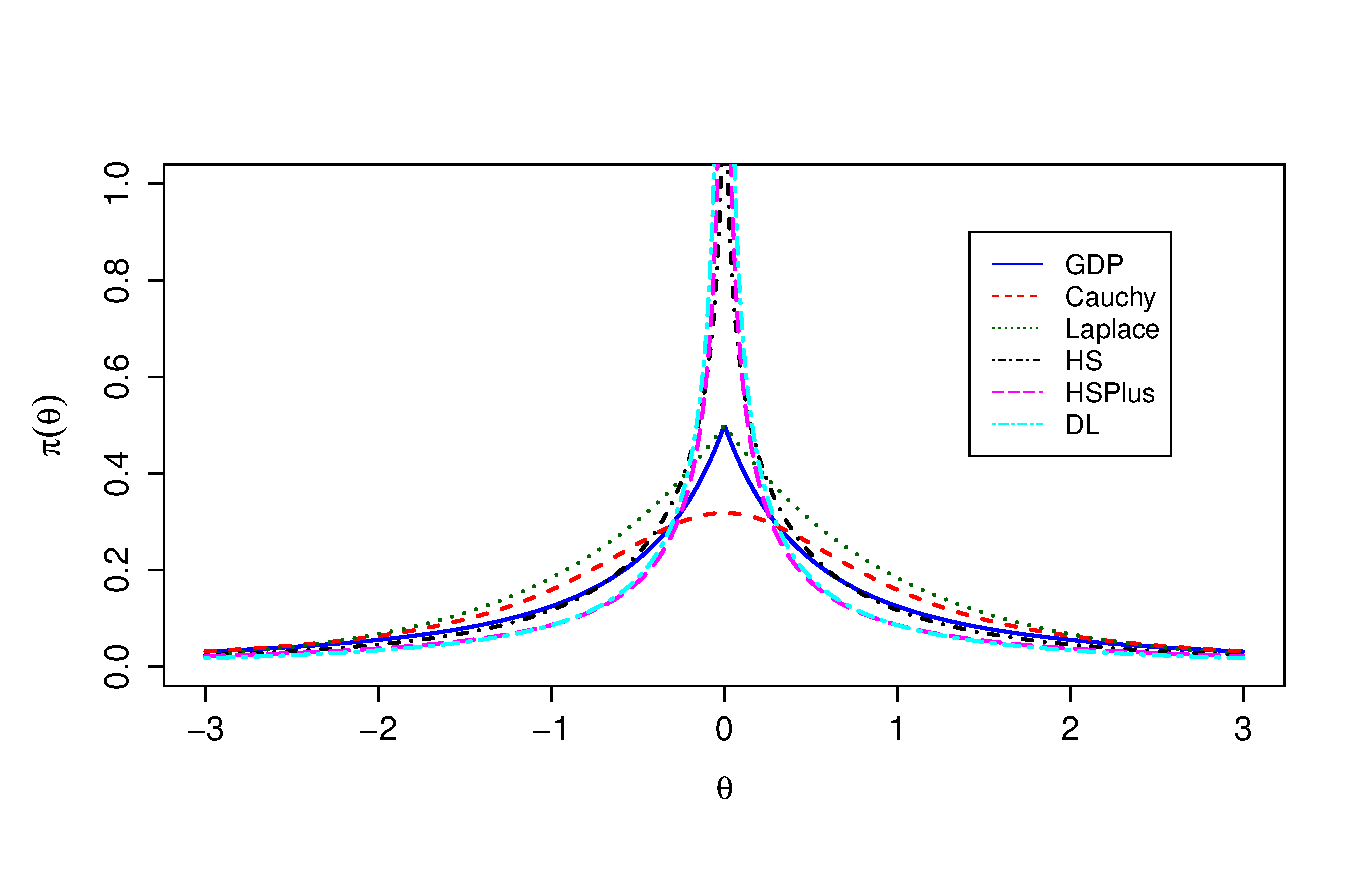
\includegraphics[width=\textwidth]{figs/densities_zero_new}%
	\caption{Marginal prior densities near the origin. The legends denote the horseshoe+ (HSPlus), horseshoe (HS), Dirichlet-Laplace (DL), generalized double Pareto (GDP), Cauchy and Laplace priors.}
	\label{fig:zero}
	\end{subfigure}
  \begin{subfigure}{0.45\linewidth}
	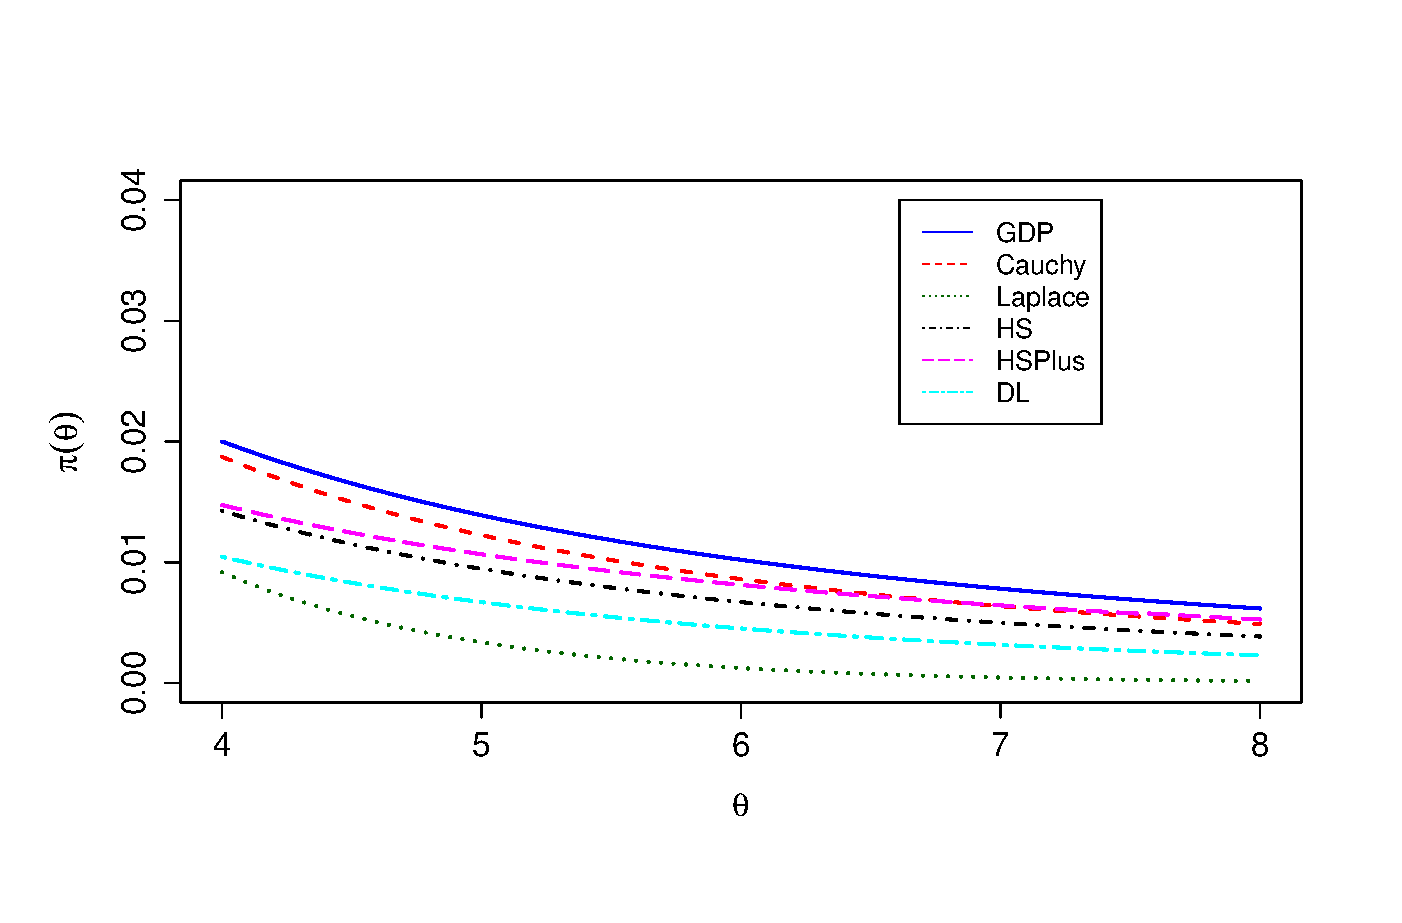
\includegraphics[width=\textwidth]{figs/densities_tails_new}
 	 \caption{Marginal prior densities in the tail regions. The legends denote the horseshoe+ (HSPlus), horseshoe (HS), Dirichlet-Laplace (DL), generalized double Pareto (GDP), Cauchy and Laplace priors.}
  \label{fig:tails}
		\end{subfigure}
\end{figure}

%\subsection{Other global-local examples}
%
%Three parameter beta \citep{armagan2011generalized}; generalized double Pareto \citep{armagan2013generalized}; generalized shrinkage prior \citep{denison12}; Dirichlet-Laplace \citep{bhattacharya2014dirichlet} ; normal-exponential-gamma \citep{griffin2005alternative}; R2-D2 \citep{zhang2016high}. 
%
   %\begin{figure}[!t]
   	%\centering
   	%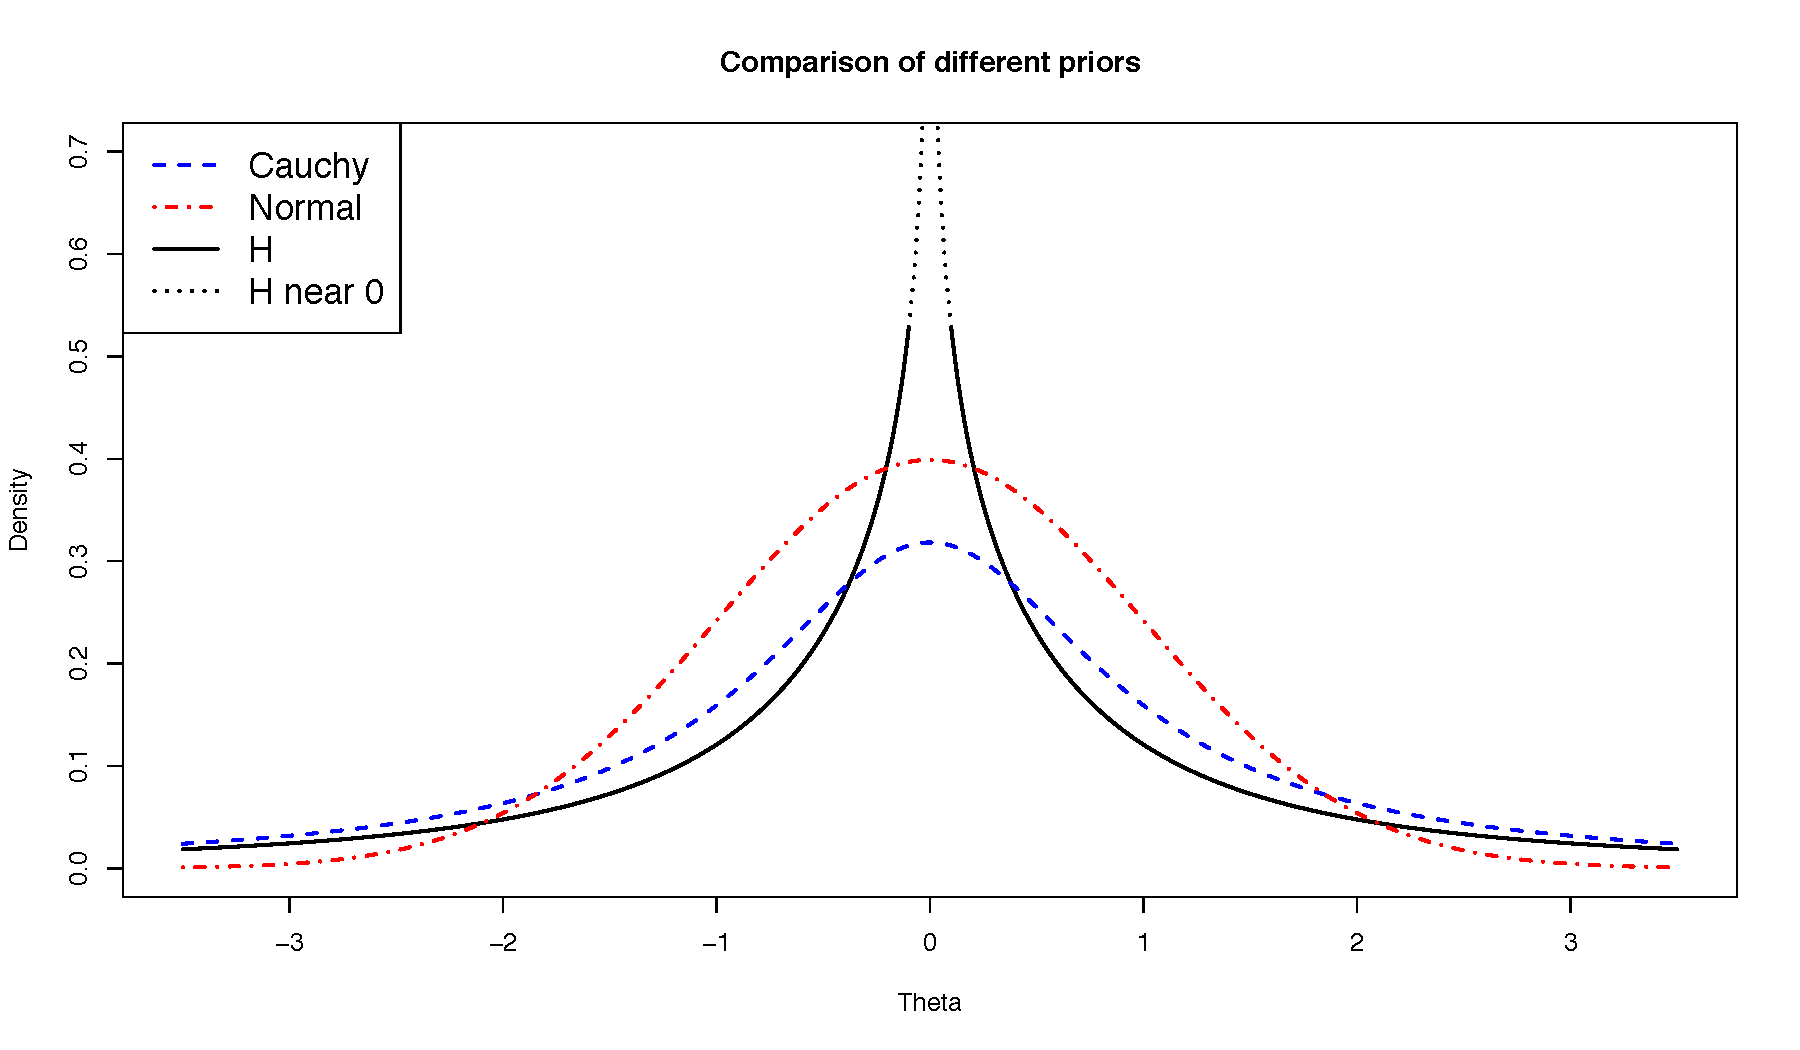
\includegraphics[width=12.5cm, height=5cm]{figs/HorseshoePrior.pdf}
   	%\caption{Horseshoe prior near zero and at the tails}
   	%\label{fig:hs}
   %\end{figure}
   %
      %\begin{figure}[!h]
   	%\centering
   	%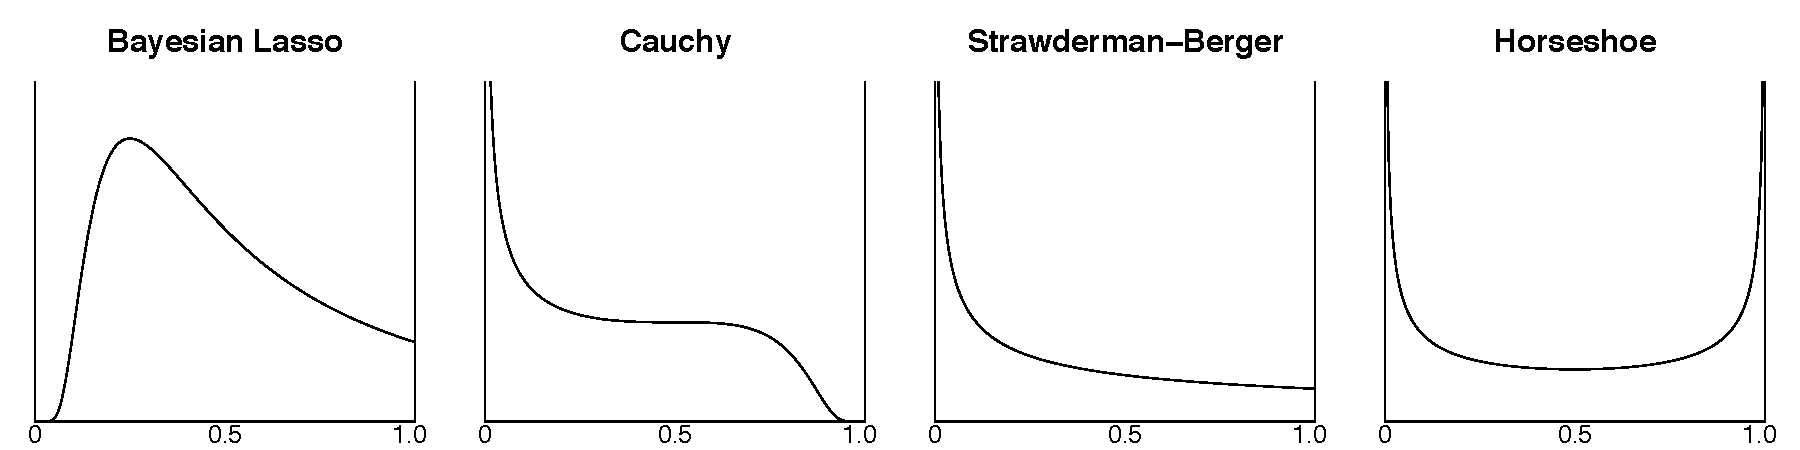
\includegraphics[width=12.5cm, height=5cm]{figs/fourkappas.pdf}
   	%\caption{Plot of kappas}
   	%\label{fig:kappa}
   %\end{figure}
   %
         %\begin{figure}[!h]
   	%\centering
   	%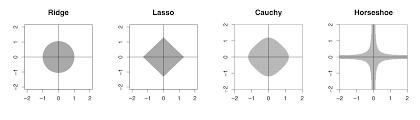
\includegraphics[width=12.5cm, height=5cm]{figs/horseshoe.png}
   	%\caption{Regularization}
   	%\label{fig:reg}
   %\end{figure}

\section{Lasso and Horseshoe}
Define estimators / compare shrinkage profiles. Asymptotic of finding zeroes. 
Explain $\phi(\theta)$ for horseshoe etc. 

\subsection{Shrinkage Profiles}
$\kappa$-scale. Figures. $p(\kappa \mid \tau)$. 


\section{Risk Calculation}

Normal means model $(y | \theta) \sim \mathcal{N} (0, \sigma^2 I_n)$. Problems with estimating $\theta$ when it is nearly black.

\subsection{Minimax $\ell_2$ risk achieved by global-local}
\begin{enumerate}
\item  \citet{van2014horseshoe} showed it for horseshoe.

\item  \citet{van2015conditions} showed it for horseshoe+ and several other ``global-local'' models.

\item \citet{ghosh14} is similar to  \citet{van2015conditions}.

\item \citet{van2016many} is a new paper that we need to read and possibly cite. 

\end{enumerate}

\subsection{Posterior Concentration and Optimal Bayes Risk}
\begin{enumerate}
%\item For spike-and-slab: \citet{bogdan2011asymptotic}.

\item For horseshoe: \citet{datta2013asymptotic}.

\item For horseshoe+: \citet{bhadra2015horseshoe+}.
\end{enumerate}

\subsection{Prediction using global-local priors}
\begin{enumerate}
\item \citet{ carvalho2010horseshoe}: K-L superefficiency for predictive density for horseshoe.


\end{enumerate}

\section{Regularisation and Hyper-parameter Selection}

Path (computational speed), Sensitivity Analysis. Cross-validation approach (has caveats), marginal MLE, $\argmax_{\tau} p(y \mid \tau)$. Plug-in estimators can be inadmissible, SURE: procedure. 


\citet{tiao65} show that the marginal likelihood, taking $ \sigma^2 = 1 $, is
$$
p( y |  \tau ) \equiv \prod_{i=1}^p ( 1 + \tau^2 )^{- \frac{1}{2}} \exp \left ( - \frac{1}{2} \sum_{i=1}^p
 \frac{ (y_i - \mu)^2 }{1 + \tau^2 } \right ) 
$$
This is positive at $ \tau = 0$. Hence the impropriety of the prior $ \tau^{-2} $ at
the origin translates to the posterior.  The marginal likelihood is decreasing at zero when the $S_i$'s are small
enough to make the exponential term nearly constant \citep{tiao65}. This is precisely the sparse coefficient case.

A number of default choices have been proposed to overcome this issues.
\citet{morris2011} propose a flat prior $ p( \tau ) \equiv 1 $. The tails of the likelihood are sufficient so as to
lead to a proper posterior. This is also related to Stein's harmonic prior 
$ || \theta ||^{-(k-2)} $ for $ k \geq 3 $.  

Methods for choosing $\tau$ will involve minimizing some criteria: %such as AIC \citep{akaike74}, BIC \citep{schwarz1978}, DIC \citep{spiegelhalter2002bayesian}, SURE \citep{stein81}, $C_p$ \citep{mallows73}. \citet{castillo2015} compared full Bayes MCMC with empirical Bayes and plug-in approaches.

\section{Simulations}
\begin{enumerate}
\item Mention R package. 

\item Compare with various methods.
\end{enumerate}

\section{Applications and Extensions}

Literature review of applications and extensions and recent development. List papers. 
Fused and group lasso. Extension to logistic (Polya-Gamma for logistic : MCMC still convex). 

\begin{enumerate}
\item \citet{bhadra2015default} use global-local priors in default Bayes Efron problems.

\item \citet{bhadra2016prediction} show how to use global-local priors for prediction. Performs better than a variety of competitors including lasso, ridge, PCR and sparse PLS.

\item \citet{datta2015inference} use global-local priors to model the rate parameter for Poisson count data.

\end{enumerate}


\section{Discussion}

What's left to do? Horseshoe subset selection. Lasso computationally quick / scalable. Horseshoe needs MCMC etc. 


\begin{enumerate}
\item So many global-local priors; what is the unifying theme?

\item How close to minimax constant can we get in estimation?

\item How close to oracle risk can we get in testing?

\item Is prediction performance optimal?

\item Yet to rigorously show global-local priors have any information theoretic properties in default Bayes problems that reference priors \citep{bernardo1979reference} enjoy.

\item \citet{bhadra2016global} demonstrate how global-local mixtures can be generated using two integral identities. This might prove useful in EM and MCMC.
\end{enumerate}

\section{Appendix: Algorithms}

Literature review of algorithms and R packages. 
LASSO: glmnet, genlasso. 
Horseshoe: horseshoe, fastHorseshoe, monomvn, our own package. 
%\section*{Appendix}
%Possibly give some R code vignette.


\section*{Other refs}

The 1988 Neyman Memorial Lecture: A Galtonian Perspective on Shrinkage Estimators - Stephen M. Stigler

\bibliographystyle{biom}
\bibliography{horseshoe-review,horseshoe-plus}

\end{document}
